\documentclass[aspectratio=169]{beamer} % includes \pause in render
% \documentclass[aspectratio=169, handout]{beamer} % do not include \pause in render

\usetheme[neutralbackground]{uniamntf}

\title[Master Colloquium Presentation]{\vspace{-2em}Classical networks for the Hubbard model with a tilted potential}
\subtitle{ - Master Thesis Colloquium - }

\author{Jonas Kell}
\institute[TP III]{Chair for theoretical Physics III}

\date[12.03.2024]{$12^{\text{th}}$ of March 2024}
% Date for the notes
\day=12\relax
\month=3\relax
\year=2025\relax

\acknowledgement{
    Jonas Kell\\
    University of Augsburg\\
    jonas.kell@student.uni-augsburg.de\\
    www.uni-augsburg.de
}

\newcommand{\blankfootnote}[1]{%
\let\thefootnote\relax\footnotetext{#1}%
}
\newcommand{\tab}{%
\,\,\,\,
}

% bibtex/biber
\usepackage[backend=biber, style=phys, biblabel=brackets]{biblatex} % citations with "modern" backend and an physics-accepted citation style
\addbibresource{literature.bib}

\newenvironment{wideitemize}{\itemize\addtolength{\itemsep}{0.3em}}{\enditemize}

%! notes control

%\setbeameroption{hide notes} % Only slides
%\setbeameroption{show only notes} % Only notes
\setbeameroption{show notes on second screen=right} % Both, use for pympress mode

% presentation tool https://github.com/Cimbali/pympress
% run: pympress colloquium-presentation.pdf 

%! notes control

% !! THIS ONLY COMPILES AFTER A SUCCESSFUL COMPILATION OF THE MAIN DOCUMENT

\begin{document}
    \begin{frame}[t,plain] 
        \maketitle
    \end{frame}

    \note[enumerate]{
        \item General notes for Master Thesis Colloquium
    }

    \begin{frame}
        \frametitle{Outline}
        \tableofcontents[pausesections] % pause toc before each section
        % \tableofcontents % all toc at once

        % toc notes do need to live inside the frame, to appear on all animated slides
        \note[item] {
            General notes during the toc slides
            \begin{itemize}
                \item TODO
            \end{itemize}
        }
    \end{frame}

    When performing time-evolution with a perturbative approach, one ought to watch out for resonances.
In the case of degenerate energy solutions, so-called \emph{secular terms} \cite{secularTermsPerturbation} might be introduced, if non-degenerate perturbation theory is used to find the solution to a degenerate problem. 
Often inaccuracies manifest as linear terms in a function where only oscillating terms would be expected.
The linear term constantly grows over time, guaranteeing the approximation is only valid for short times and then diverges further and further from the exact solution.

For the examined Hamiltonian the first occurrence of such terms can be spotted in the second order cumulant expansion of the Hamiltonian.
\autoref{eq:time-ordered-integral-part1} and \autoref{eq:time-ordered-integral-part2} specifically list extra solutions for the cases where the two energies are the same.
This resonance causes a linear term to appear in the expansion, while all other pre-factors so far were complex exponentials -- meaning they are oscillating.

The idea to combat this is to replace the perturbative parameters that were calculated analytically with variational parameters instead.
This has the motive to generate a physically motivated structure, but the fine details of the parameter weights are adjusted by optimization.
E.g. for the \emph{neural-network quantum state} \cite{neuralNetworkQuantumStates} approach, a neural network structure is used to represent a wave-function.
Reason for this being the hope that the exponentially complicated wave-function can be expressed as a \glqq higher truth\grqq{} only requiring few parameters to describe a seemingly complicated wave-function.
While it would be basically impossible to always find the few-parameter-solution, \emph{approximating} it close enough with optimization akin to machine-learning should be a suitable replacement.

The following section aims to achieve better approximations than the ones found by cumulant expansion by letting the parameters be optimized during the step to reflect the situation more closely.
    \section{Time Evolution}

    \begin{frame}[t]
        \frametitle{Goal of the Calculation}

        \begin{itemize}
            \item Evaluate the time-evolution of the system for various observables \pause
            \begin{itemize}
                \item Uses calculation in the \emph{Interaction Picture} \pause
                \item Introduce operator-less \emph{effective Hamiltonian}
            \end{itemize}
        \end{itemize}

        \vspace{1cm}

        \makebox[\textwidth][c]{
            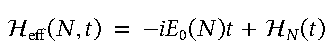
\includegraphics[width=0.165\textwidth,page=1]{main-content/time-evolution/effective-hamiltonian-definition.pdf}
            \includegraphics[width=0.45\textwidth,page=2]{main-content/time-evolution/effective-hamiltonian-definition.pdf}
        }

        % notes 
        \onslide % on all slides of frame
        \note[item] {
            Goal: evaluate the time-evolution for different observables (effectively)
        }
        \note[item] {
            Brute-force calculation is at least NP-hard, definitely exponential and one of the hardest problems to solve computationally generally
        }
        \note[item] {
            Strategy: perform a controlled expansion in the perturbation V and re-express the formulas as a dependency on a operator-free "effective Hamiltonian"
            \begin{itemize}
                \item Can be re-ordered without concern as no operators
                \item For the re-formulation we will use the interaction picture
            \end{itemize}
        }
    \end{frame}

    \begin{frame}[t]
        \frametitle{The effective Hamiltonian}

        \makebox[\textwidth][c]{
            \includegraphics[width=0.55\textwidth,page=3]{main-content/time-evolution/effective-hamiltonian-definition.pdf}
        }

        \pause
        \begin{itemize}
            \item Constructed from the contributions of the base energy and the perturbation \pause
            \item Base energy contribution:
        \end{itemize}

        \makebox[\textwidth][c]{
            \includegraphics[width=0.65\textwidth,page=4]{main-content/time-evolution/effective-hamiltonian-definition.pdf}
        }

        % notes 
        \onslide % on all slides of frame
        \note[item] {
            Comprised of two parts:
            \begin{itemize}
                \item Simple, quickly stated term that depends on the base energy 
                \item Complicated one that will be expanded in the perturbation
            \end{itemize}
        }
    \end{frame}

    \begin{frame}[t]
        \frametitle{The effective Hamiltonian}

        \begin{itemize}
            \item To evaluate the time-evolution of the perturbation
        \end{itemize}

        \makebox[\textwidth][c]{
            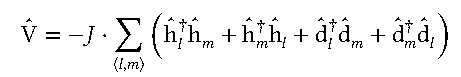
\includegraphics[width=0.50\textwidth,page=1]{main-content/time-evolution/v-in-interaction.pdf}
        }

        \pause
        \begin{itemize}
            \item Solve the equation of motion for the ladder operators
        \end{itemize}
        
        \vspace{-0.1cm}
        \makebox[\textwidth][c]{
            \includegraphics[width=0.50\textwidth,page=2]{main-content/time-evolution/v-in-interaction.pdf}
        }


        % notes 
        \onslide % on all slides of frame
        \note[item] {
            Need: V-Operator in the Interaction picture 
        }
        \note[item] {
            For that: first solve the equations of motion for the ladder operators and the plug in
        }
        \note[item] {
            Solving the equations of motions in the interaction picture requires their number operator being \emph{idempotent}
        }
    \end{frame}

    \begin{frame}[t]
        \frametitle{The effective Hamiltonian}

        \begin{itemize}
            \item Insert and reorder the operators
        \end{itemize}

        \makebox[\textwidth][c]{
            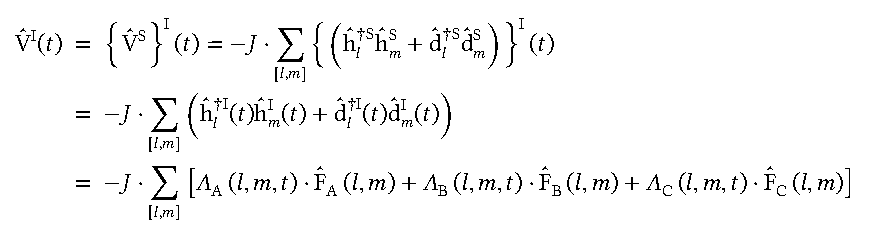
\includegraphics[width=0.80\textwidth,page=1]{main-content/time-evolution/v-in-interaction-solution.pdf} % TODO
        }%
        \vspace{-0.0cm}
        \pause
        \makebox[\textwidth][c]{
            \includegraphics[width=0.80\textwidth,page=2]{main-content/time-evolution/v-in-interaction-solution.pdf}
        }

        % notes 
        \onslide % on all slides of frame
        \note[item] {
            Inserting yields TWO kinds of terms
            \begin{itemize}
                \item time-dependent analytical pre-factors (or their integral as one sees later)
                \item dressed hopping terms, basically only depending on the occupation of the state N
            \end{itemize}
        }
    \end{frame}

    \begin{frame}[t]
        \frametitle{The effective Hamiltonian}

        \begin{itemize}
            \item Evaluate the contribution to the effective Hamiltonian \pause
            \begin{itemize}
                \item Requires previously calculated value of the V-operator in the Interaction Picture \pause
                \item Controllable \emph{cumulant expansion}
            \end{itemize}
        \end{itemize}

        \pause[2]
        \vspace{0.2cm}
        \makebox[\textwidth][c]{
            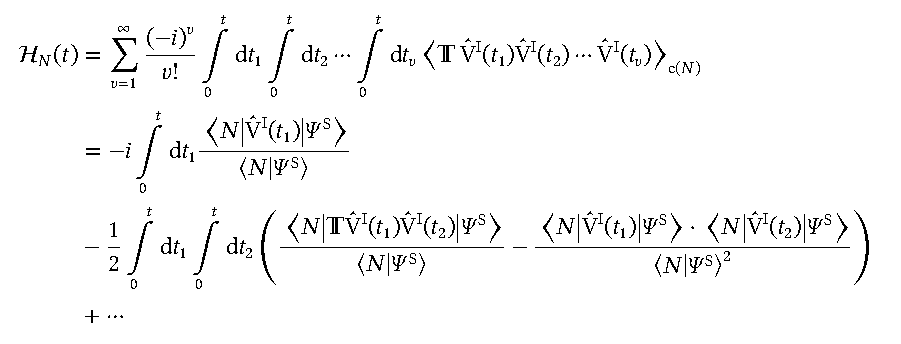
\includegraphics[width=0.80\textwidth,page=1]{main-content/time-evolution/effective-hamiltonian-n.pdf}
        }

        % notes 
        \onslide % on all slides of frame
        \note[item] {
            Generally any expansion possible, but here we expand the \emph{argument of the exponential} - cumulant
        }
        \note[item] {
            first order easily derivable with the info from the previous slide (integrate)
        }
        \note[item] {
            second and higher orders very complicated occupation terms and the pre-factors require quite a lot of edge-cases to integrate with the time-ordering operator
            \begin{itemize}
                \item Hint onto the thesis for this exact derivation
            \end{itemize}
        }
    \end{frame}

    \begin{frame}[t]
        \frametitle{Handling of Observables}

        \begin{itemize}
            \item This allows for general evaluation of expectation values \pause
            \begin{itemize}
                \item Requires a probability for the state
                \item Requires a local observable
            \end{itemize}
        \end{itemize}

        \pause[1]
        \vspace{0.2cm}
        \makebox[\textwidth][c]{
            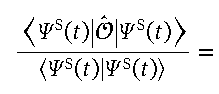
\includegraphics[width=0.28\textwidth,page=1]{main-content/time-evolution/time-evolution-of-observable.pdf}
        }
        \pause[2]
        \makebox[\textwidth][c]{
            \includegraphics[width=0.80\textwidth,page=2]{main-content/time-evolution/time-evolution-of-observable.pdf}
        }

        % notes 
        \onslide % on all slides of frame
        \note[item] {
            Why? General evaluation of an expectation value for an observable.
            \begin{itemize}
                \item Probability for state
                \item Local observable (can be swapped for many different ones)
            \end{itemize}
        }
        \note[item] {
            Does ONLY require difference of effective Hamiltonian for evaluation (notice for later)
        }
    \end{frame}

    \begin{frame}[t]
        \frametitle{Simple Observables}

        \begin{itemize}
            \item Local observable for double occupation measurement \pause
            \begin{itemize}
                \item Observables generally are very sparse matrices
                \item Reduces to pure occupation measurement
            \end{itemize}
        \end{itemize}

        \makebox[\textwidth][c]{
            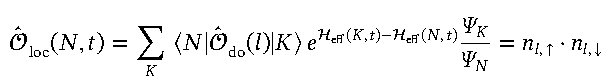
\includegraphics[width=0.7\textwidth,page=1]{main-content/time-evolution/local-observables-simple-ops.pdf}
        }

        \pause
        \begin{itemize}
            \item Local observable for particle current measurement \pause
            \begin{itemize}
                \item Requires evaluation of the difference of two effective Hamiltonians
            \end{itemize}
        \end{itemize}

        \makebox[\textwidth][c]{            
            \includegraphics[width=0.8\textwidth,page=2]{main-content/time-evolution/local-observables-simple-ops.pdf}
        }

        % notes 
        \onslide % on all slides of frame
        \note[item] {
            Complex valued observable, make sure this cancels in the case of approximations
        }
        \note[item] {
            \emph{SHOULD MENTION:} Energy and variance (most expensive ones, are assumed to keep constant, can be used to gauge the quality of the expansion)
        }
    \end{frame}

    \begin{frame}[t]
        \frametitle{Access to Density-Matrics}

        \begin{itemize}
            \item Non-classical (\emph{quantum}) measurements depend on the (reduced) density matrix \pause
                \begin{itemize}
                    \item Access to \emph{purity}, \emph{concurrence} and other entanglement measures/monotones\pause
                \end{itemize}
            \item Direct calculation not possible
        \end{itemize}

        \vspace{-0.2cm}
        \makebox[\textwidth][c]{
            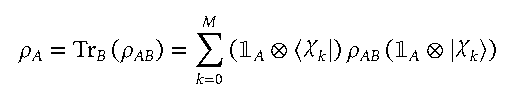
\includegraphics[width=0.65\textwidth,page=1]{main-content/time-evolution/reduced-density-matrix.pdf}
        }

        \vspace{-0.2cm}
        \pause
        \begin{itemize}
            \item Use Pauli matrices to expand the complex 4x4 matrix
        \end{itemize}

        \makebox[\textwidth][c]{
            \includegraphics[width=0.65\textwidth,page=2]{main-content/time-evolution/reduced-density-matrix.pdf}
        }

        % notes 
        \onslide % on all slides of frame
        \note[item] {
            Quite interesting, because of this extra mentioned the Pauli operators
        }
        \note[item] {
            No access to the full density matrix, can not trace out, because too many states to trace out
        }
        \note[item] {
            BUT: as the complex 4x4 matrix can be written in the base of the kronecker product of two pauli matrices, can be expressed (because the pauli operators can be translated into hard-core bosonic ones again and for these we have the general fromula for expectation values)
        }
    \end{frame}

    \begin{frame}[t]
        \frametitle{Access to Density-Matrics}

        \makebox[\textwidth][c]{
            \includegraphics[width=0.75\textwidth,page=3]{main-content/time-evolution/reduced-density-matrix.pdf}
        }

        % notes 
        \onslide % on all slides of frame
        \note[item] {
            Sixteen terms (with missing cases trivially derived from the ones that are given)
        }
        \note[item] {
            Again all depend on the difference of effective hamiltonians between two states ith local modifications
        }
    \end{frame}
    \section{Sampling \& Simplifications}
    \begin{frame}[t]
        \frametitle{Probability Calculations}
        
        \vspace{-0.6cm}

        \begin{columns}[t]
            \column{0.4\textwidth}
                \begin{itemize}
                    \item Full probability still requires normalization \pause
                    \item Switch to the Metropolis \emph{Hastings} algorithm
                    \begin{itemize}
                        \item Non-exponential number of samples \pause
                        \item Depends only on a transition probability
                        \item Does not need normalization because it cancels
                    \end{itemize}
                \end{itemize}
    
            \onslide
            \column{0.4\textwidth}
                \vspace{0.0cm}
                \pause[3]
                \makebox[\textwidth][c]{
                    \includegraphics[width=1.3\textwidth,page=2]{main-content/simplifications/mc-sampling.pdf}
                }
    
        \end{columns}

        \pause[2]
        \vspace{0.15cm}
        \makebox[\textwidth][c]{
            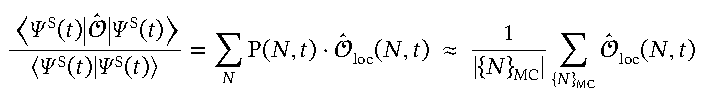
\includegraphics[width=0.80\textwidth,page=1]{main-content/simplifications/mc-sampling.pdf}
        }

        % notes 
        \onslide % on all slides of frame
        \note[item] {
            Normalization requires knowing exponential amount of states and we need to sample an exponential amount to get all
        }
        \note[item] {
            switch to METROPOLIS HASTINGS algorithm
            \begin{itemize}
                \item only fixed number of samples required (depends on the desired precision)
                \item No normalization needed, because it cancels in the division
            \end{itemize}
        }
    \end{frame}

    \begin{frame}[t]
        \frametitle{Analytical Simplifications}
        
        \begin{itemize}
            \item Choose a helpful initial state
        \end{itemize}
    
        \pause
        \vspace{-0.35cm}
        \makebox[\textwidth][c]{
            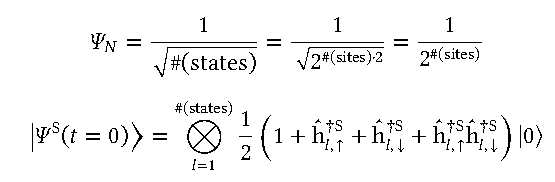
\includegraphics[width=0.60\textwidth,page=1]{main-content/simplifications/analytical-simplification-example.pdf}
        }

        \vspace{-0.1cm}
        \begin{itemize}
            \item Now \emph{almost all} terms cancel in \emph{differences} of the effective Hamiltonian \pause
            \begin{itemize}
                \item Exemplary for single flip on base energy term
            \end{itemize} 
        \end{itemize}

        \vspace{-0.15cm}
        \makebox[\textwidth][c]{
            \includegraphics[width=0.62\textwidth,page=2]{main-content/simplifications/analytical-simplification-example.pdf}
        }

        % notes 
        \onslide % on all slides of frame
        \note[item] {
            Choose the helpful \emph{initial state} with all base states having the same probability
        }
        \note[item] {
            because of this the divisions of Psi-N over Psi-K everywhere give 1 and many terms cancel (outside of the local interaction ragne of the modificaiton)
        }
    \end{frame}

    \section{Variational Classical Networks}
    \begin{frame}[t]
        \frametitle{Why and How should Parameters be variational?}

        \vspace{-0.6cm}
        \begin{columns}[t]
            \column{0.4\textwidth}
                \begin{itemize}
                    \item Theoretically: always better approximation through higher order terms \pause
                    \begin{itemize}
                        \item Hard to calculate analytically and expensive to evaluate \pause
                    \end{itemize}
                    \item Hope: Better behavior if parameters are \emph{learned}/\emph{optimized}, starting from the analytical result \pause
                \end{itemize}
    
            \column{0.4\textwidth}
                \vspace{-0.3cm}
                \makebox[\textwidth][c]{
                    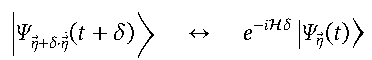
\includegraphics[width=0.95\textwidth,page=1]{main-content/variational-classical-networks/variational-classical-networks-theory.pdf}
                }
                \pause
                \makebox[\textwidth][c]{
                    \includegraphics[width=0.7\textwidth,page=2]{main-content/variational-classical-networks/variational-classical-networks-theory.pdf}
                }%
                \pause
                \vspace{1cm}
                \makebox[\textwidth][c]{
                    \includegraphics[width=1.1\textwidth,page=3]{main-content/variational-classical-networks/variational-classical-networks-theory.pdf}
                }
                \pause
                \makebox[\textwidth][c]{
                    \includegraphics[width=0.7\textwidth,page=4]{main-content/variational-classical-networks/variational-classical-networks-theory.pdf}
                }
    
        \end{columns}
        
        % notes 
        \onslide % on all slides of frame
        \note[item] {
            Argument:
            \begin{itemize}
                \item Could go on performing the controlled expansion for all perturbation-strengths and get nice result
                \item But higher orders complicated and expensive
                \item Try to get more from the lower orders, by using Variational parameters (optimized by the problem, we hope they can incorperate influence from higher order terms without them being present)
            \end{itemize}
        }
        \note[item] {
            Time dependent variational principle (TDVP)
            \begin{itemize}
                \item Find a parametrized \emph{wavefunction}
                \item Update the parameters so that a tiny nudge into the direction of the \emph{time DERIVATIVE} of the parameter vector has the same effect as a time evolution with the full hamiltonian
                \item The first order numerical integration (could do higher orders, but for the concept here)
            \end{itemize}
        }
        \note[item] {
            O: Variational derivative\,\,\,            E: local energy (we had already earlier)
        }
    \end{frame}


    \begin{frame}[t]
        \frametitle{Why and How should Parameters be variational?}

        \vspace{-0.6cm}
        \begin{columns}[t]
            \column{0.4\textwidth}
                \begin{itemize}
                    \item Theoretically: always better approximation through higher order terms
                    \begin{itemize}
                        \item Hard to calculate analytically and expensive to evaluate
                    \end{itemize}
                    \item Hope: Better behavior if parameters are \emph{learned}/\emph{optimized}, starting from the analytical result
                \end{itemize}
    
            \column{0.4\textwidth}
                \vspace{-0.3cm}
                \makebox[\textwidth][c]{
                    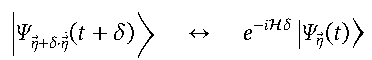
\includegraphics[width=0.95\textwidth,page=1]{main-content/variational-classical-networks/variational-classical-networks-theory.pdf}
                }
                \makebox[\textwidth][c]{
                    \includegraphics[width=0.7\textwidth,page=2]{main-content/variational-classical-networks/variational-classical-networks-theory.pdf}
                }%
                \pause
                \vspace{0.5cm}
                \makebox[\textwidth][c]{
                    \includegraphics[width=1.1\textwidth,page=5]{main-content/variational-classical-networks/variational-classical-networks-theory.pdf}
                }%
                \pause
                \vspace{0.15cm}
                \makebox[\textwidth][c]{
                    \includegraphics[width=0.6\textwidth,page=6]{main-content/variational-classical-networks/variational-classical-networks-theory.pdf}
                }
    
        \end{columns}
        
        % notes 
        \onslide % on all slides of frame
        \note[item] {
            Pseudo inversion
        }
        \note[item] {
            S: covariance matrix
        }
        \note[item] {
            F: TDVP force
        }
        \note[item] {
            \emph{time DERIVATIVE}
        }
    \end{frame}

    \begin{frame}[t]
        \frametitle{First Try: Cumulant Expansion Prefactors}

        \begin{itemize}
            \item Idea: generate a variational Hamiltonian by replacing the analytical prefactors
        \end{itemize}
        \vspace{-0.2cm}
        \makebox[\textwidth][c]{
            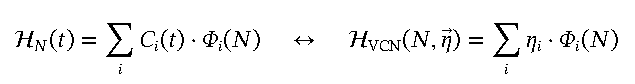
\includegraphics[width=0.7\textwidth,page=1]{main-content/variational-classical-networks/variational-classical-networks-application.pdf}
        }%
        \vspace{0.4cm}
        \pause
        \makebox[\textwidth][c]{
            \hspace{-1.5cm}
            \makebox[0.5\textwidth][c]{
                \includegraphics[width=0.5\textwidth,page=2]{main-content/variational-classical-networks/variational-classical-networks-application.pdf}%
            }
            \makebox[0.5\textwidth][c]{
                \raisebox{0.55cm}{
                    \includegraphics[width=0.5\textwidth,page=3]{main-content/variational-classical-networks/variational-classical-networks-application.pdf}
                }
            }
        }
        
        % notes 
        \onslide % on all slides of frame
        \note[item] {
            Idea: replace prefactors that depend on the time and keep the shape of teh terms that depend on the occupation of the state
        }
        \note[item] {
            Verification: as the TDVP is also derived from an \emph{action principle} that must mean as per noethers theorem that the energy MUST be conserved by a correct TDVP step
        }
    \end{frame}

    \begin{frame}[t]
        \frametitle{Correction: Watch Explicit Time-Dependency}

        \begin{itemize}
            \item First strategy is not suitable
            \begin{itemize}
                \item Energy- and variance is not conserved
            \end{itemize}
            \pause
            \item Problem: explicit time-dependency of base energy
        \end{itemize}

        \makebox[\textwidth][c]{
            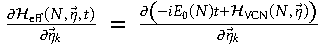
\includegraphics[width=0.55\textwidth,page=1]{main-content/variational-classical-networks/variational-classical-networks-application-explicit.pdf}
        }

        \pause
        \begin{itemize}
            \item Solution: Replace base energy factors with variational parameters
        \end{itemize}

        \makebox[\textwidth][c]{
            \includegraphics[width=0.3\textwidth,page=3]{main-content/variational-classical-networks/variational-classical-networks-application-explicit.pdf}
            \raisebox{1cm}{
                \includegraphics[width=0.62\textwidth,page=2]{main-content/variational-classical-networks/variational-classical-networks-application-explicit.pdf}
            }
        }
        
        % notes 
        \onslide % on all slides of frame
        \note[item] {
            Fails because not taken the explicit time-dependency into account as it was \emph{differentiated away} wrongfully 
        }
        \note[item] {
            As a solution: introduce variational base-energy factors - which is a successful strategy
        }
    \end{frame}

    \section{Implementation \& Experiments}
    \begin{frame}[t]
        \frametitle{Implementation}
        
        \begin{itemize}
            \item Too much code to properly show 
            \begin{itemize}
                \item Look at repository for overview
            \end{itemize}
            \pause
            \item Testing: validation code to check the correct implementation
            \begin{itemize}
                \item Independent implementations for same functionality
                \item Sanity checks for state of data and program
            \end{itemize}
            \pause
            \item Optimization: runtime comparison for different code styles
            \begin{itemize}
                \item For generated code fast execution over readability
            \end{itemize}
        \end{itemize}

        % notes 
        \onslide % on all slides of frame
        \note[item] {
            While nothing is looked at in detail maybe interesting for some
        }
        \note[item] {
            Testing: validation and assertion based programming
        }
        \note[item] {
            Optimization: code style runtime experiments
        }
    \end{frame}

    \begin{frame}[t]
        \frametitle{Numerical Experiments}
        
        \begin{itemize}
            \item Sadly no presentation possible in the small time allocated for the presentation
            \item The plots are in the presentation in the supplementary material
        \end{itemize}

        \makebox[\textwidth][c]{\includegraphics[width=0.6\textwidth]{./../thesis-latex/plotgeneration/concurrence-from-spin/concurrence-comparison.pdf}}

        % notes 
        \onslide % on all slides of frame
        \note[item] {
            See supplementary material for more plots and stuff
        }
    \end{frame}

    \section{Conclusion \& Outlook}
    \begin{frame}[t]
        \frametitle{Conclusion \& Outlook}
        
        \begin{exampleblock}{Conclusion:}
            \begin{itemize}
                \item Successfully transferred and validated the theory
                \item Working implementation
                \begin{itemize}
                    \item Extensively tested
                    \item Configurable and extensible
                \end{itemize}
                \item Started validating expectations with measurements on the compute cluster
            \end{itemize}
        \end{exampleblock}
        
        \pause

        \begin{block}{Outlook:}
            \begin{itemize}
                \item Re-write in lower level language to gain performance over Python
                \item Start more real experiments now that the theory is validated to work
            \end{itemize}
        \end{block}

        % notes 
        \onslide % on all slides of frame
        \note[item] {
            Conclusion:
            \begin{itemize}
                \item Managed to Solve all problems 
                \item Provide heavily \emph{tested} and \emph{extensible} library of code AND theoretical summary
                \item Started to validate expectations with computations on the cluster
            \end{itemize}
        }
        \note[item] {
            Future plans:
            \begin{itemize}
                \item re-write in performant language after testing is successful
                \item Go through the parameters to start investigating the behavior of the systems
            \end{itemize}
        }
    \end{frame}


    \section*{Summary \& Conclusion}
    {
        \setbeamertemplate{frametitle}[uniamntfack] % use the acknowledgment-style for this slide
        \begin{frame}[plain]{Acknowledgment}
            \vspace{1cm}

            Thank you for your kind attention\\

            \vspace{1cm}
            \makebox[0.4\textwidth][c]{
                
\includegraphics[width=0.3\textwidth]{extra-slides/qr-github.png}
            }
        \end{frame}
    }

    \note[enumerate]{
        \item Thank you for your kind attention
        \item All tools and other resources are referenced in the presentation
        \item You can also find everything on my Github
    }

    \begingroup % group to not count pages from here
        \begin{frame}[allowframebreaks,noframenumbering]
            \frametitle{References}
            \nocite{*}
            \printbibliography[title={Bibliography}]
        \end{frame}
        
        \section*{Extra slides}
            
\begin{frame}[noframenumbering]{Extra Plots: Overview}
    \begin{itemize}
        \item \hyperlink{plot:exact-comparison}{Exact comparison density matrix}
        \item \hyperlink{plot:energy-variance}{First orders: energy and variance comparison}
        \item \hyperlink{plot:j-sweep}{J parameter sweep}
        \item \hyperlink{plot:mc-convergence}{Monte Carlo sampling convergence}
        \item \hyperlink{plot:runtime-comparison}{Runtime validation}
    \end{itemize}
\end{frame}

\begin{frame}[noframenumbering]{Exact Comparison: Concurrence}
    \label{plot:exact-comparison}
    \vspace{-0.4cm}
    \makebox[\textwidth][c]{\includegraphics[height=.8\paperheight]{./../thesis-latex/plotgeneration/concurrence-from-spin/concurrence-comparison.pdf}}
    \note[item]{
        Concurrence comparison of small system with exact calculations and comparison thereof
    }
    \note[item]{
        See extreme boost of second order 
    }
\end{frame}
\begin{frame}[noframenumbering]{Exact Comparison: Purity}
    \vspace{-0.4cm}
    \makebox[\textwidth][c]{\includegraphics[height=.8\paperheight]{./../thesis-latex/plotgeneration/concurrence-from-spin/purity-comparison.pdf}}
    \note[item]{
        Purity measurements for the graph of the measurement from one page before
    }
\end{frame}
\begin{frame}[noframenumbering]{Exact Comparison: Pauli Measurements}
    \vspace{-0.6cm}
    \makebox[\textwidth][c]{\includegraphics[height=.83\paperheight]{./../thesis-latex/plotgeneration/concurrence-from-spin/pauli-measurements.pdf}}
    \note[item]{
        Portrait mode format, because extracted from the thesis. 
    }
    \note[item]{
        You can see what a problem the z-contributions are
    }
\end{frame}

\begin{frame}[noframenumbering]{First Orders: Energy Comparison}
    \label{plot:energy-variance}
    \vspace{-0.4cm}
    \makebox[\textwidth][c]{\includegraphics[height=.8\paperheight]{./../thesis-latex/plotgeneration/energy-variance/energy.pdf}}
    \note[item]{
        Second picture zoomed in
    }
\end{frame}
\begin{frame}[noframenumbering]{First Orders: Variance Comparison}
    \vspace{-0.4cm}
    \makebox[\textwidth][c]{\includegraphics[height=.8\paperheight]{./../thesis-latex/plotgeneration/energy-variance/variance.pdf}}
    \note[item]{
        Second picture zoomed in
    }
\end{frame}

\begin{frame}[noframenumbering]{J-Sweep: Current Border}
    \label{plot:j-sweep}
    \vspace{-0.4cm}
    \makebox[\textwidth][c]{\includegraphics[height=.8\paperheight]{./../thesis-latex/plotgeneration/j-sweep/current-border.pdf}}
    \note[item]{
        Logarithmic plot
    }
    \note[item]{
        Measurements show the trend of the convergence of the relative error for small perturbations
    }
    \note[item]{
        Depends on the observable though, still
    }
\end{frame}
\begin{frame}[noframenumbering]{J-Sweep: Current Center}
    \vspace{-0.4cm}
    \makebox[\textwidth][c]{\includegraphics[height=.8\paperheight]{./../thesis-latex/plotgeneration/j-sweep/current-center.pdf}}
\end{frame}
\begin{frame}[noframenumbering]{J-Sweep: Single Occupation Center}
    \vspace{-0.4cm}
    \makebox[\textwidth][c]{\includegraphics[height=.8\paperheight]{./../thesis-latex/plotgeneration/j-sweep/single-occ-center.pdf}}
\end{frame}
\begin{frame}[noframenumbering]{J-Sweep: Double Occupation Border}
    \vspace{-0.4cm}
    \makebox[\textwidth][c]{\includegraphics[height=.8\paperheight]{./../thesis-latex/plotgeneration/j-sweep/double-occ-border.pdf}}
\end{frame}

\begin{frame}[noframenumbering]{Monte Carlo Convergence: Occupation}
    \label{plot:mc-convergence}
    \vspace{-0.4cm}
    \makebox[\textwidth][c]{\includegraphics[height=.8\paperheight]{./../thesis-latex/plotgeneration/monte-carlo-variance-test/occupation.pdf}}
    \note[item]{
        Well as we can see, the appriximation converges as the variance gos to zero
    }
\end{frame}
\begin{frame}[noframenumbering]{Monte Carlo Convergence: Occupation}
    \vspace{-0.4cm}
    \makebox[\textwidth][c]{\includegraphics[height=.8\paperheight]{./../thesis-latex/plotgeneration/monte-carlo-variance-test/spin-current.pdf}}
\end{frame}

\begin{frame}[noframenumbering]{Runtime Validation}
    \label{plot:runtime-comparison}
    \vspace{-0.4cm}
    \makebox[\textwidth][c]{\includegraphics[height=.8\paperheight]{./../thesis-latex/plotgeneration/runtime-complexity/runtime.pdf}}
\end{frame}

% \makebox[\textwidth][c]{\includegraphics[height=.8\paperheight]{./../thesis-latex/plotgeneration/vcn-eff-stepsize/}}
% \makebox[\textwidth][c]{\includegraphics[height=.8\paperheight]{./../thesis-latex/plotgeneration/vcn-energy-conservation/}}
% \makebox[\textwidth][c]{\includegraphics[height=.8\paperheight]{./../thesis-latex/plotgeneration/vcn-square-comparison/}}
% \makebox[\textwidth][c]{\includegraphics[height=.8\paperheight]{./../thesis-latex/plotgeneration/vcn-square-small/}}
% \makebox[\textwidth][c]{\includegraphics[height=.8\paperheight]{./../thesis-latex/plotgeneration/system-size-dependency/}}

% \begin{frame}[noframenumbering]{}
%     \label{plot:exact-comparison}
%     \vspace{-0.4cm}
%     \note[item]{
%     }
% \end{frame}
    \endgroup

\end{document}
